\documentclass[UTF8]{article}

\setlength{\parindent}{0pt}
\setlength{\parskip}{1ex plus 0.5ex minus 0.2ex}

% define the title
\author{H.~Partl}
\title{Minimalism}
\usepackage{amsfonts}
\usepackage{amsmath}
\usepackage{latexsym}
\usepackage{amssymb}
\usepackage{makeidx}
\usepackage{hep}
\usepackage{graphicx,graphics,color}

\makeindex

\newcommand{\txsit}[1]
{This is the \emph{#1} Short
	Introduction to \LaTeXe}

% preamble
\newtheorem{law}{Law}
\newtheorem{jury}[law]{Jury}

\newtheorem{mur}{Murphy}[subsection]

\begin{document}
{\,{\rm GeV}}


\[\begin{aligned}
x={}& a+b+c+{} \\
&d+e+f+g
\end{aligned}\]

\[\begin{aligned}
x =& a+b+c+{} \\
&d+e+f+g
\end{aligned}\]

\[\begin{aligned}
x ={}& a+b+c+ \\
&d+e+f+g
\end{aligned}\]

ams,xc

ams, xc

ams,   xc

\begin{equation}
	dssdf\\
	sdfasd\\
	safsd
\end{equation}
\[
\lVert
\rVert
\]

Fig.~1

Fig.1

Fig.Apple

Fig. Apple

Fig.\ Apple

Fig\@. Apple
\section{safsd}
\begin{align}
&\begin{aligned}
\Gamma^{\mu}[a,p]=
-(D+F)^2\,I[a,N,\pi]-
\frac{(3F+D)^2}{6}\,I[a,K,\Lambda]-
\frac{(D-F)^2}{2}\,I[a,K,\Sigma]
\end{aligned}\\
&\begin{aligned}
\Gamma^{\mu}[a,n]=(D+F)^2\,I[a,N,\pi]-
(D-F)^2\,I[a,K,\Sigma]
\end{aligned}
\end{align}

\[
\slashed{{p'}}
\]

\[
\slashed{p}^\prime
\]

\begin{figure}[htbp]
	\centering
	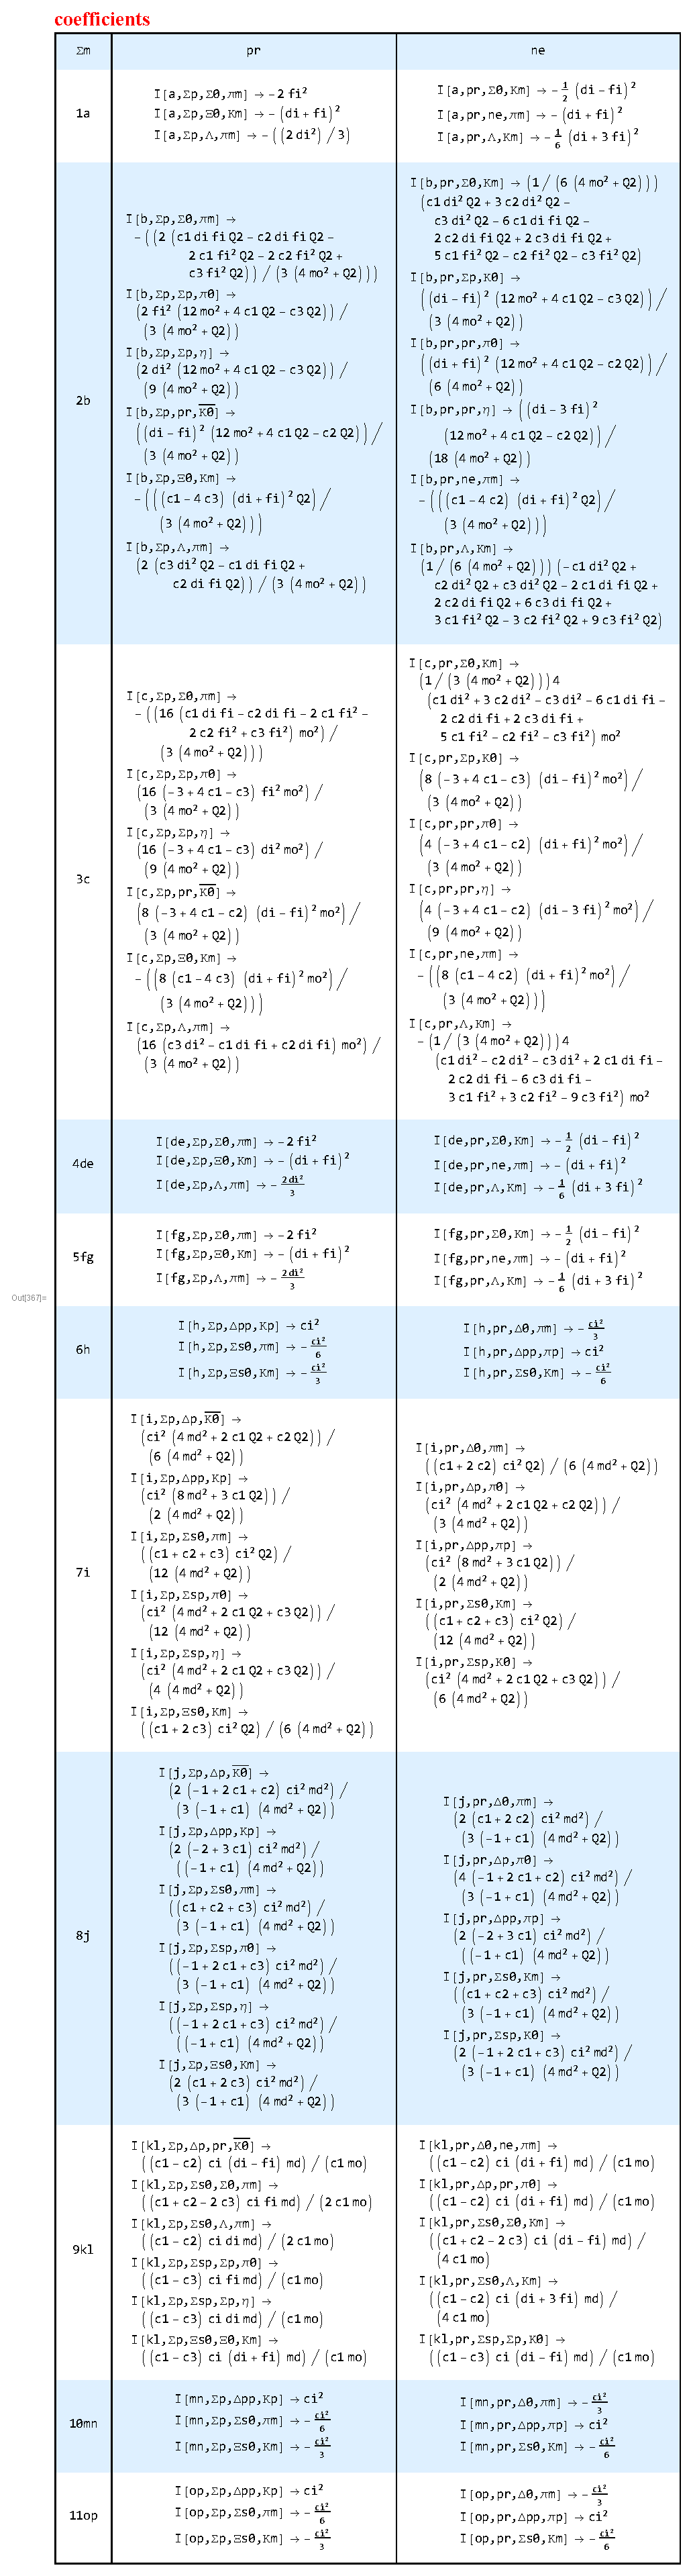
\includegraphics[height=\textheight,width=\textwidth]{coe.all.eps}
	\caption{asd.}
	\label{fig:loop8}
\end{figure}





\end{document}